\section{Introduction to Ridge Regression}

\subsection{Ordinary Least squares Method}
Suppose that we have input vector \(\xB = (x_1, x_2, \dots, x_p)^\top\) and want
to predict a real-valued output \(y\). The linear regression model has the from
\begin{equation}\label{eq:lin-reg}
    f(\xB) = \beta + \sum_{j=1}^p x_j w_j = \linearprod{\wB}{\xB'},
\end{equation}
in which \(\wB = (\beta, w_1, \dots, w_p)^\top \in \R^{p+1}\) and 
\(\xB' = (1, x_1, \dots, x_p)^\top \in \R^{p+1}\). The linear model either assumes that
the regression function is linear, or that the linear model is reasonable approximation.
Here \(\wB\) is unknown parameter vector.

\begin{figure}[!htbp]
    \centering
    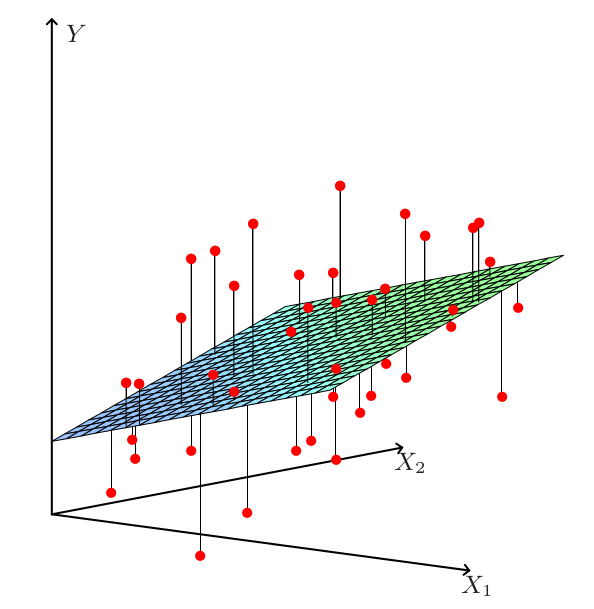
\includegraphics[scale = 0.3]{fig/linear-model.png}
    \caption{Linear model fitting with \(\xB \in \R^2\).}
    \label{fig:linear-model}
\end{figure}

Generally speaking we have a training dataset with training data \((\xB_1, y_1), \dots, 
(\xB_N, y_N)\) from which we would like to estimate the parameter vector \(\wB\), and
\(\xB_i = (x_{i1}, x_{i2}, \dots, x_{ip})^\top\).
If we use \emph{Ordinary Least Squares} (OLS) method, we will pick the \(\wB\) which can
minimize \emph{the residual sum of squares} (RSS)
\begin{equation}\label{eq:RSS-OLS}
    \begin{aligned}
        \RSS (\wB) &= \sum_{i=1}^N (y_i - f(\xB_i))^2 \\
        &= \sum_{i=1}^N \left( y_i - \beta - \sum_{j=1}^p x_{ij}w_j \right)^2.
    \end{aligned}
\end{equation}

Denote by \(\bm{X} \in \R^{N \times (p + 1)}\) the matrix with each row an input vector, and similarly, let 
\(\yB \in \R^N\) be the output vector in this training dataset. Then we can rewritte Eq (\ref{eq:RSS-OLS}) in
as
\begin{equation}\label{eq:RSS-OLS-mat}
    \RSS(\wB) = (\yB - \bm{Xw})^\top(\yB - \bm{Xw}) 
\end{equation}
This is a quadratic function. Differentiating with respect to \(\wB\) we can get 
\begin{equation}
    \begin{aligned}
        \pdv{\RSS}{\wB} &= -2 \bm{X}^\top (\yB - \bm{Xw}) \\
        \pdv{\RSS}{\wB}{\wB^\top} &= 2\bm{X}^\top \bm{X}.
    \end{aligned}
\end{equation}
Suppose that \(\bm{X}\) has full column rank. Therefore, \(\bm{X}^\top\bm{X}\) is positive definite.
We can set the first derivative to \(0\)
\begin{equation}
    \bm{X}^\top (\yB - \bm{X\beta}) = 0
\end{equation}
to get the unique solution
\begin{equation}\label{eq:solution-OLS}
    \hat{\wB}_{\text{OLS}} = \left(\bm{X}^\top \bm{X}\right)^{-1} \bm{X}^\top \yB.
\end{equation}

\subsection{Ridge Regression}
However, according to Eq (\ref{eq:solution-OLS}), \(\hat{\wB}_{\text{OLS}}\) depends on \(\bm{X}^\top\bm{X}\). 
In some cases, \(\bm{X}^\top\bm{X}\) may be \emph{singular} or \emph{nearly singular}. 
When there are many correlated variables in a linear regression model, their coefficients can become poorly determined and
exhibit high variance. In those cases, we call \(\bm{X}\) \emph{ill-conditioned}.
Small changes to elements of \(\bm{X}\) will lead to large changes in \(\bm{X}^\top\bm{X}\). In addition, \(\hat{\wB}_{\text{OLS}}\) may provide a 
good fit to the training data, but it will not fit sufficiently well to the test data.

In order to alleviate this problem, we introduce \emph{ridge regression}. Ridge regression shrinks the regression coefficients by imposing a penalty 
on their size. The ridge coefficients minimize a penalized residual sum of squares,
\begin{equation}\label{eq:beta-rigde}
    \hat{\wB}_{\text{ridge}} = \mathop{\arg\min}_{\wB} \left\{
        \sum_{i=1}^N \left(
            y_i - \beta - \sum_{j=1}^p x_{ij} w_j 
        \right)^2 + \lambda \sum_{j=1}^p w_j^2
    \right\}. 
\end{equation}
Here \(\lambda \ge 0\) is a \emph{complexity parameter} that controls the amount of shrinkage.

Rewriting the criterion in Eq (~\ref{eq:beta-rigde}) in matrix form, we can obtain
\begin{equation}
    \RSS = (\yB - \bm{Xw})^\top (\yB - \bm{Xw}) + \lambda \wB^\top \wB,
\end{equation}
and
\begin{equation}\label{eq:ridge-derivative}
    \begin{aligned}
        \pdv{\RSS}{\wB} &= -2\bm{X}^\top (\yB - \bm{Xw}) + 2\lambda\wB\\
        \pdv{\RSS}{\wB}{\wB^\top} &= 2\bm{X}^\top\bm{X} + 2\lambda \bm{I}.
    \end{aligned}
\end{equation}
Let the first derivative in Eq (\ref{eq:ridge-derivative}) be zero, then the ridge regression solution can be expressed as 
\begin{equation}
    \hat{\wB}_{\text{ridge}} = \left( \bm{X}^T \bm{X} + \lambda \bm{I} \right)^{-1} \bm{X}^\top \bm{y},
\end{equation}
where \(\bm{I}\) is the \((p+1) \times (p+1)\) \emph{identity matrix}.
The solution adds a positive constant to the diagonal of \(\bm{X}^\top \bm{X}\) before inversion, which makes this problem
nonsigular, even if \(\bm{X}^\top \bm{X}\) is not of full rank.

\begin{figure}[!htbp]
    \centering
    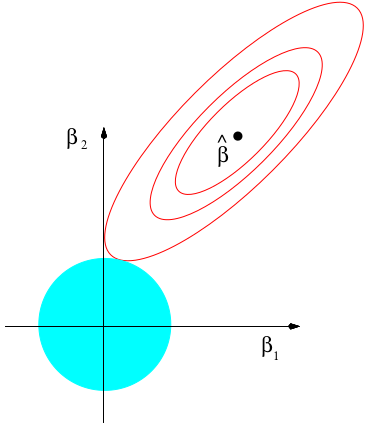
\includegraphics[scale = 0.4]{fig/ridge-reg.png}
    \caption{Estimation picture for ridge regression.}
    \label{fig:ridge-reg}
\end{figure}